\documentclass[12pt, a4 paper]{article}
\usepackage{babel}
\usepackage{graphicx, hyperref, xcolor, fancyhdr, amssymb, amsmath, amsthm, mdframed, tikz}
\usepackage{mathrsfs}
\usepackage[acronym, toc]{glossaries}
\usepackage{pdfpages}
\usepackage{svg}
\usepackage{algorithmic}
\usepackage[ruled, linesnumbered]{algorithm2e}


% editorial comments in the text or in marginal notes
% 1st argument: initials of the person making the comment,
% 2nd argument: comment to insert
\long\def\ednote#1#2{\par\noindent\framebox{\begin{minipage}{.98\linewidth}\linespread{.7}\footnotesize #1: #2\end{minipage}}\par}
\newcommand{\edmargin}[2]{\marginpar{\raggedright\linespread{.7}\tiny #1: #2}}

% redefine proof environment with grey background and black square at the end
\renewenvironment{proof}[1][Proof]{\begin{mdframed}[backgroundcolor=black!5, topline=false, rightline=false, bottomline=false, linecolor=black!15, linewidth=3pt]{\noindent\textit{#1.}\ }}{\noindent\hfill$\blacksquare$\end{mdframed}}

% \usepackage{times}

\hypersetup{
    colorlinks,
    linkcolor={red!60!black},
    citecolor={blue!80!black},
    urlcolor={blue!80!black}
}

% \pagestyle{fancy}
% \renewcommand\headrulewidth{.5pt}
% \fancyhead[L]{
%     V. Trélat
% }

% \fancyhead[C]{
%     \textbf{Verification in Isabelle/HOL of Hopcroft's algorithm for minimizing DFAs including runtime analysis}
% }

% \fancyhead[R]{
%     % Current section
%     \ifnum\c@secnumdepth>0
%         \thesection
% }

% theorems
\theoremstyle{definition}
\newtheorem{theorem}{Theorem}
\newtheorem{lemma}{Lemma}
\newtheorem{remark}{Remark}
\newtheorem{definition}{Definition}
\newtheorem{requirement}{Requirement}

% Glossary

\makeglossaries

% \newacronym{tiaa}{TIAA}{This Is An Acronym}

\begin{document}

\begin{titlepage}
    \begin{center}
        \vfill
        
\includegraphics[height=1.5cm]{img/logoTUM.png}
        \hfill
        
\includegraphics[height=1.5cm]{img/logoartem.png}
        \hfill
        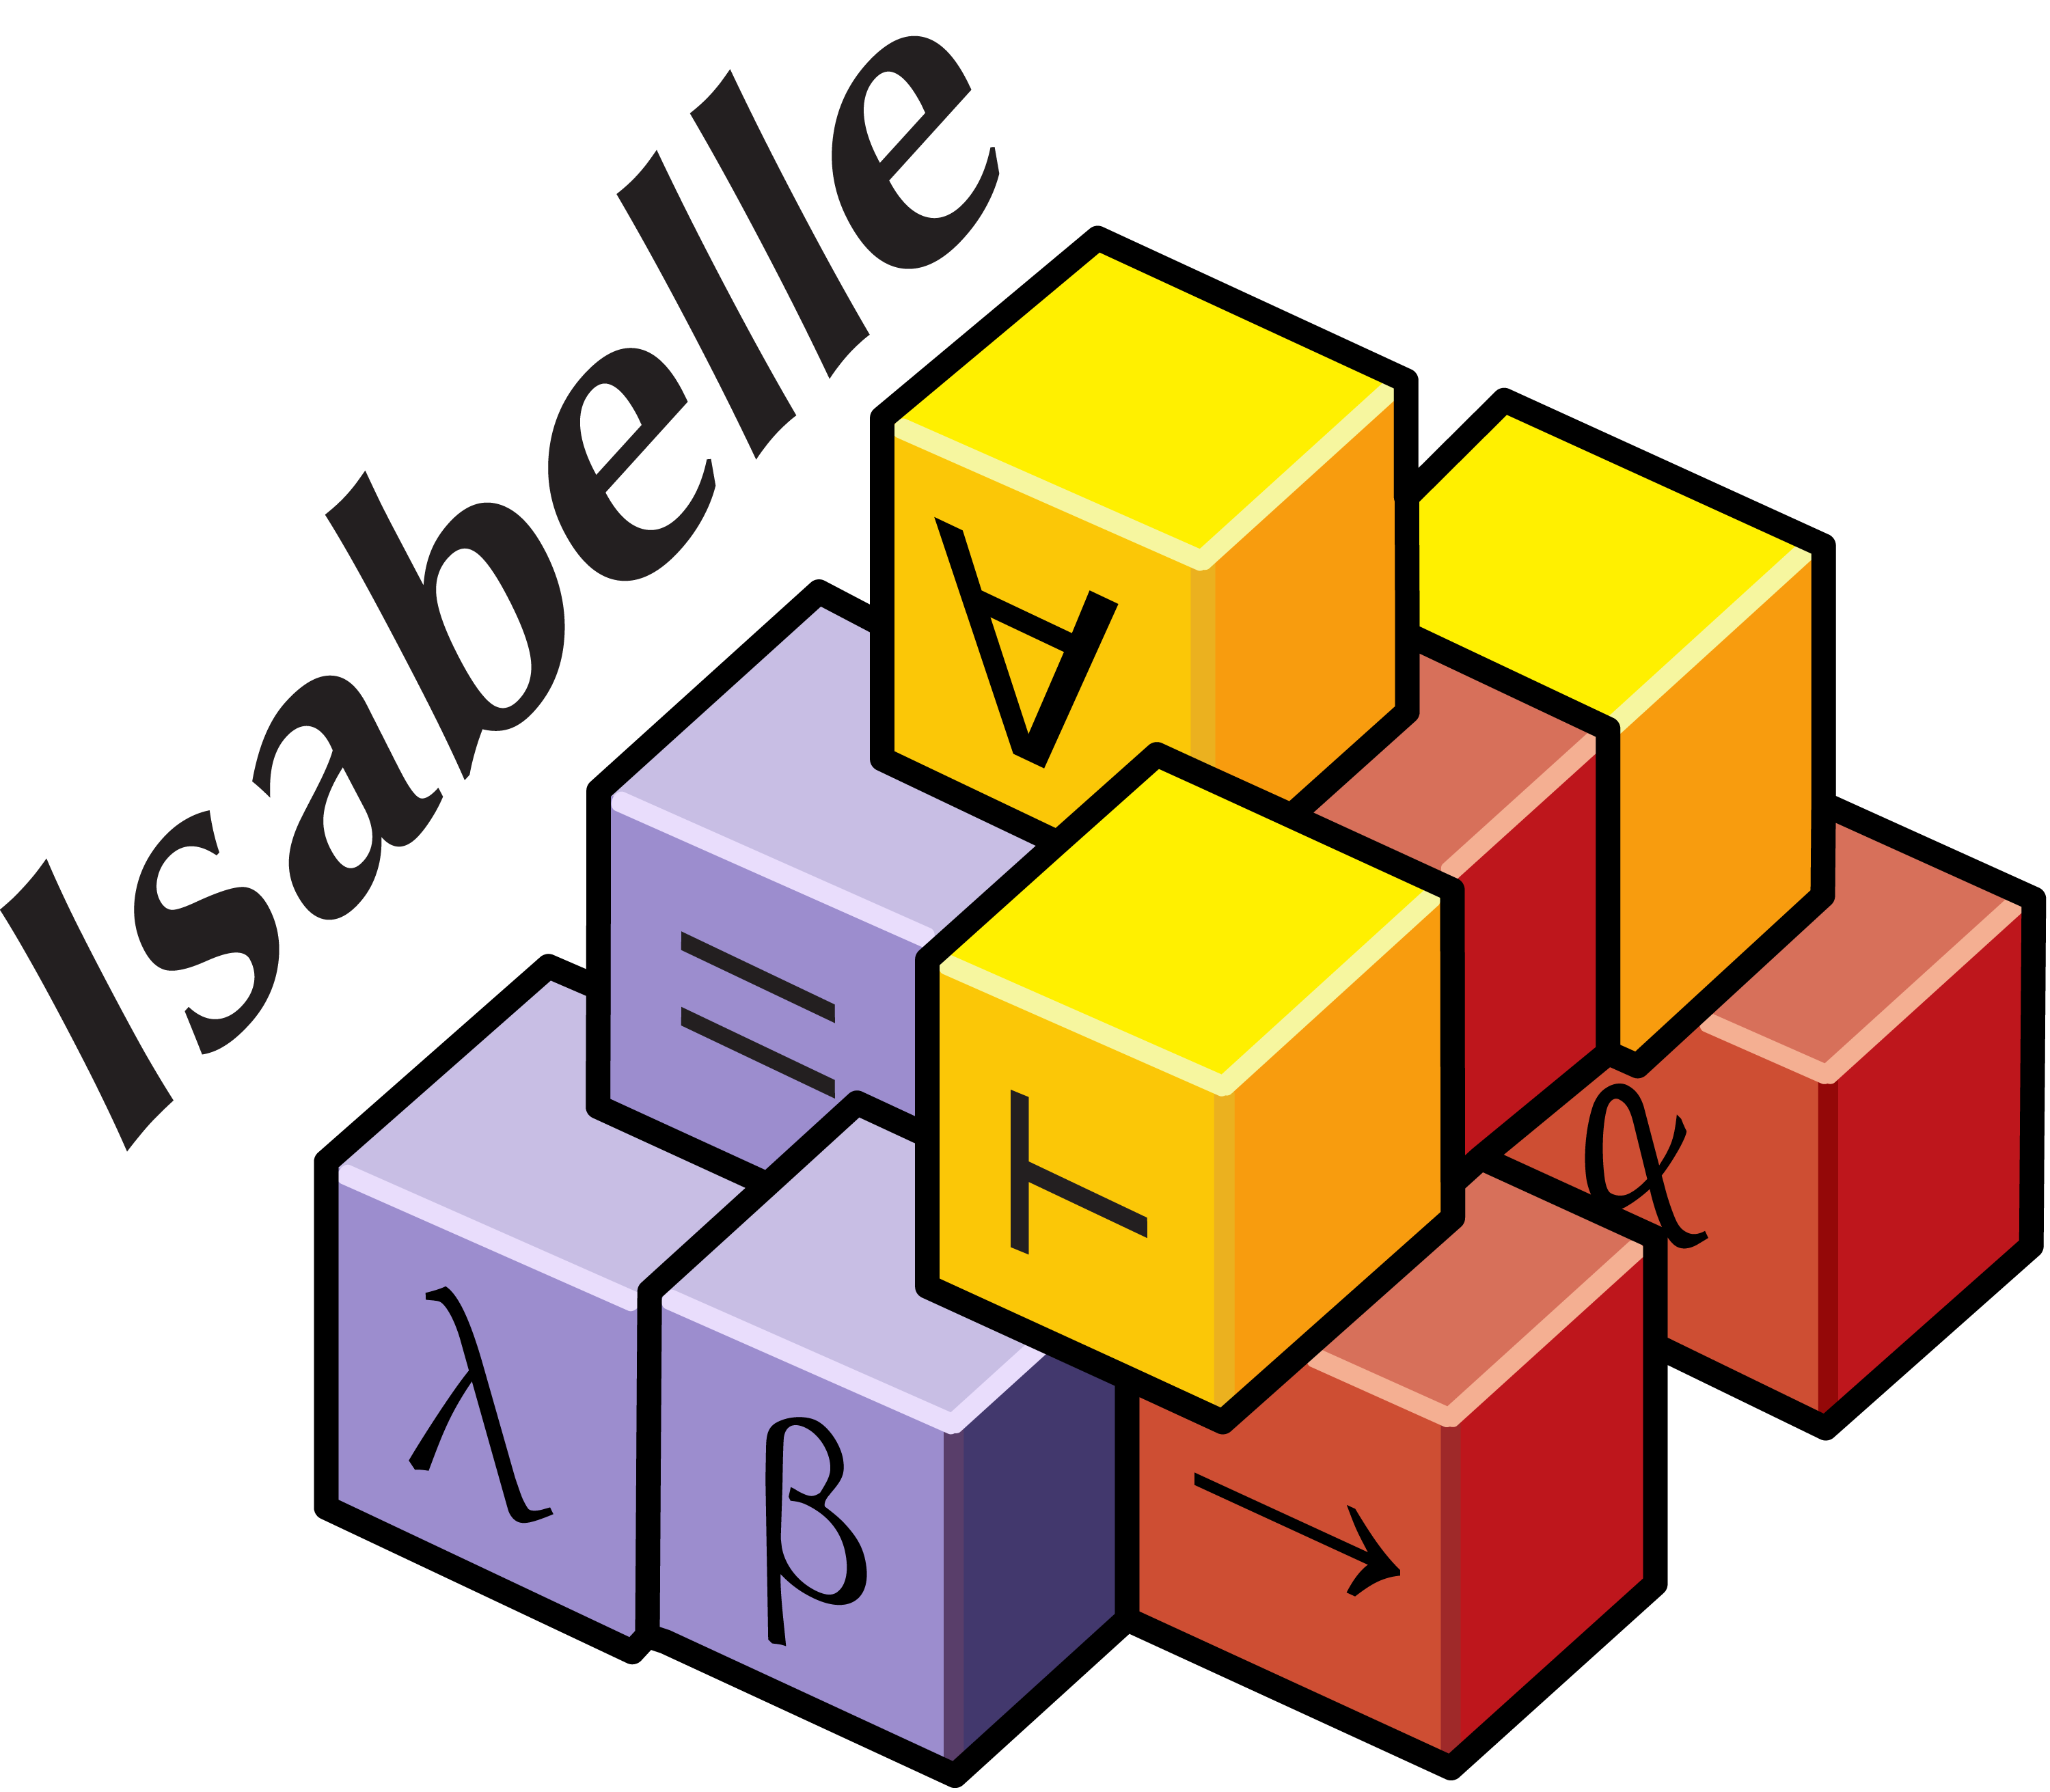
\includegraphics[height=1.5cm]{img/logoisabelle.png}
        \vfill
    \end{center}
    \begin{center}
        
        \textbf{Final year intership report}
        \vfill

        \large{\textbf{Verification in Isabelle/HOL of Hopcroft's algorithm for minimizing DFAs including runtime analysis}}
    \end{center}
    
    \vfill
    
    \begin{center}
        \textbf{Vincent Trélat}\\
        \vspace{1cm}
        \textit{\today}
    \end{center}
    \vfill
    \begin{center}
        
\includegraphics[height=1.2cm]{img/logoGE.png}
        \hfill
        
\includegraphics[height=1.2cm]{img/logoUL.png}
    \end{center}
\end{titlepage}

\tableofcontents

\pagebreak

\section{Introduction}
\subsection{Original algorithm}
John E. Hopcroft's algorithm for minimizing DFAs was first presented in his original 1971 paper \cite{Hop71} as a formal algorithm. Algorithm~\ref{alg:original} is a direct translation of the original algorithm with only slight changes in the notations.

\begin{algorithm}[H]
\SetAlgoLined
\caption{Hopcroft's original formal algorithm}
\label{alg:original}
\KwData{\textbf{Input:} a finite DFA $\mathcal{A} = (\mathcal{Q}, \Sigma, \delta, q_0, \mathcal{F})$}
\KwResult{\textbf{Output:} the equivalence class of $\mathcal{Q}$ under state equivalence}
Construct $\delta^{-1}(q, a) := \{t \in \mathcal{Q}\ |\ \delta(t, a) = q\}$ for all $q \in \mathcal{Q}$ and $a \in \Sigma$ \;\label{alg:original:1}
Construct $P_1 := \mathcal{F}$, $P_2 := \mathcal{Q} \setminus \mathcal{F}$ and $a_i := \{q \in P_i \ | \ \delta^{-1}(q, a) \neq \varnothing \}$ for all $i \in \{1, 2\}$ and $a \in \Sigma$ \;
Let $k := 3$ \;
For all $a \in \Sigma$, construct $L_a := \underset{0 \leq i < k}{\operatorname*{arg\,min}}\ \left| a_i \right|$ \; \label{alg:original:4}
\While{$\exists a \in \Sigma, L_a \neq \varnothing$\label{alg:original:loop}}{
    Pick $a \in \Sigma$ such that $L_a \neq \varnothing$ and $i \in L_a$ \;
    $L_a := L_a \setminus \{i\}$ \;
    \ForAll{$j < k, \exists q \in P_j, \delta(q, a) \in a_i$}{
        $P'_j := \{t \in P_j\ |\ \delta(t, a) \in a_i \}$ and $P''_j := P_j \setminus P'_j$ \;
        $P_j := P'_j$ and $P_{k} := P''_j$; construct $a_j$ and $a_k$ for all $a \in \Sigma$ accordingly \;
        For all $a \in \Sigma$, $L_a := \begin{cases}
        L_a \cup \{j\} & \text{if $j \notin L_a \land \left| a_j \right| \leq \left| a_k \right|$} \\
        L_a \cup \{k\} & \text{otherwise}
        \end{cases}$ \;
        $k := k + 1$ \;
    }
}
\end{algorithm}

\subsection{Modern formalisation}

Today, the algorithm is usually given in a more mathematical and formalised way\footnote{see for example \cite{esparza2023automata}}, as presented below in Algorithm~\ref{alg:modern}.

\begin{definition}
    Let $\mathcal{A} = (Q, \Sigma, \delta, q_0, I, F)$ be a DFA. Let $P$ be a partition of $Q$. Let $B \in P$ and $a \in \Sigma$. We say for $C \in P$ that
    $(a, C)$ splits $B$ if $$\exists q_1, q_2 \in B \quad \delta(q_1, a) \in C \land \delta(q_2, a) \notin C.$$
\end{definition}

If $(a, C)$ is a splitter of $B$, $P$ can be updated to $P \setminus \{B\} \cup \{B', B''\}$, where $$B' := \{q \in B \ | \ \delta(q, a) \in C\} \text{ and } B'' := B \setminus B'.$$

\begin{algorithm}[H]
\SetAlgoLined
\caption{Hopcroft's algorithm in a modern style}
\label{alg:modern}
\KwData{\textbf{Input:} a finite DFA $\mathcal{A} = (\mathcal{Q}, \Sigma, \delta, q_0, \mathcal{F})$}
\KwResult{\textbf{Output:} the language partition $P_\ell$}
\eIf{$\mathcal{F} = \varnothing \lor \mathcal{Q} \setminus \mathcal{F} = \varnothing$}{
    \Return $\mathcal{Q}$
}{
    $P := \{ \mathcal{F}, \mathcal{Q} \setminus \mathcal{F} \}$ \;
    $\mathcal{W} := \{ (a, \min \{ \mathcal{F}, \mathcal{Q} \setminus \mathcal{F}\}, a \in \Sigma \}$ \;
    \While{$\mathcal{W} \neq \varnothing$}{
        Pick $(a, B')$ from $\mathcal{W}$ \;
        \ForAll{$B \in P$}{
            Split $B$ with $(a, B')$ into $B_0$ and $B_1$ \;
            $P := (P \setminus \{B\}) \cup \{B_0, B_1\}$ \;
            \ForAll{$b \in \Sigma$}{
                \eIf{$(b, B \in \mathcal{W})$}{
                    $\mathcal{W} := (\mathcal{W} \setminus \{(b, B)\}) \cup \{(b, B_0), (b, B_1)\}$ \;
                }{
                    $\mathcal{W} := \mathcal{W} \cup \{(b, \min \{ B_0, B_1 \})\}$ \;
                }
            }
        }
    }
}

\end{algorithm}

\section{Proof of correctness}
\section{Time complexity analysis}

We focus on the original algorithm presented in Algorithm~\ref{alg:original} in order to work on the arguments given in \cite{Hop71}. The data structures used at that time were mostly linked lists, but let us rather give some requirements for the data structures instead of actual implementations. The goal is to show that the algorithm can be executed in $O(m \cdot n \log n)$ time, where $m$ is the number of symbols in the alphabet and $n$ is the number of states in the DFA.

The following requirements come directly from \cite{Hop71} and are specific to the algorithm presented in Algorithm~\ref{alg:original}.

\begin{requirement}
    \label{req:1}
Sets such as $\delta^{-1}(q, a)$ and $L_a$ must be represented in a way that allows $O(1)$ time for addition and deletion in front position.
\end{requirement}

\begin{requirement}
    \label{req:2}
Vectors must be maintained to indicate whether a state is in a given set.
\end{requirement}

\begin{requirement}
    \label{req:3}
Sets such as $P_i$ must be represented in a way that allows $O(1)$ time for addition and deletion at any given position.
\end{requirement}

\begin{requirement}
    \label{req:4}
For a state $q$ in a set $P_i$ or $a_i$, its position must be determined in $O(1)$ time.
\ednote{VT}{Maybe not necessary? This should be provable from Req.\ \ref{req:2} and Req.\ \ref{req:3}.}
\end{requirement}

\begin{lemma}
    Lines \ref{alg:original:1} to \ref{alg:original:4} can be executed in $O(\left| \Sigma \right| \cdot \left| \mathcal{Q} \right|)$ time.
\end{lemma}
\begin{proof}
    The non trivial part is the computation of the inverse transition function $\delta^{-1}(q, a)$, for all $q \in \mathcal{Q}$ and $a \in \Sigma$. This can be done in $O(\left| \Sigma \right| \cdot \left| \mathcal{Q} \right|)$ time by iterating over $\Sigma$ and traversing the automaton (e.g.\ with a DFS) and keeping track of the predecessor at each step.
\end{proof}

\begin{lemma}
    An iteration of the loop at line \ref{alg:original:loop} taken for a letter $a$ and an index $i \in L_a$ takes a time proportional to the number of transitions terminating in $P_i$ and the number of symbols in the alphabet, i.e. $\Theta\left(\left| \Sigma \right| \cdot \left| \bigcup_{q \in P_i} \delta^{-1}(q, a) \right| \right)$ time.
\end{lemma}
\begin{proof}
    We pick an $a \in \Sigma$ such that $L_a \neq \varnothing$ and an $i \in L_a$. We need to examine all $j < k$ such that $\exists q \in P_j, \delta(q, a) \in a_i$ to construct the sets corresponding to splitting the block $P_j$ w.r.t.\ $a$ and $P_i$.

    Let $j < k$. From the definition of $a_i$, we obtain the following:
    \begin{align*}
        \exists q \in P_j, \delta(q, a) \in a_i &\iff \exists q \in P_j, \delta(q, a) \in P_i \land \underset{\text{true}}{\underbrace{\delta^{-1}(\delta(q, a), a) \neq \varnothing}} \\
        & \iff \exists q \in P_j, \delta(q, a) \in P_i
    \end{align*}
    Which corresponds to finding states in $P_j$ having an outgoing $a$-transition to a state in $P_i$, as represented in the following scheme:
    \begin{center}
        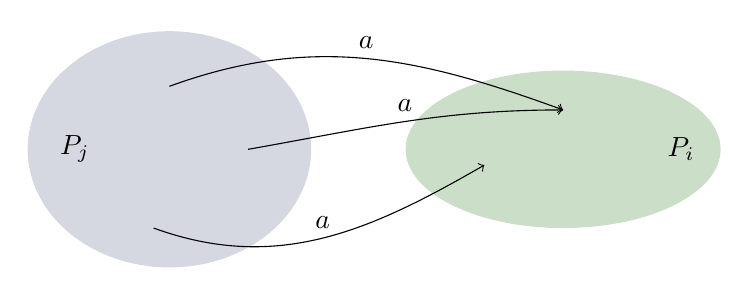
\begin{tikzpicture}
            \definecolor{color1}{RGB}{213, 216, 224}
            \definecolor{color2}{RGB}{202, 222, 200}
            
            \fill[color=color1] (0,0) ellipse (1.8cm and 1.5cm);
            \fill[color=color2] (5,0) ellipse (2cm and 1cm);
            
            \node at (-1.2,0) {$P_j$};
            \node at (6.5,0) {$P_i$};

            \draw[->] (0, 0.8) to[in=160, out=20] node[above]{$a$} (5,0.5);
            \draw[->] (1,0) to[in=180, out=10] node[above]{$a$} (5,0.5);
            \draw[->] (-.2,-1) to[in=210, out=-20] node[above]{$a$} (4,-.2);
        \end{tikzpicture}
    \end{center}
    This set of states can be expressed via the inverse transition function:
    $$ \{q \in P_j\ |\ \delta(q,a) \in P_i \} = \left( \bigcup_{q \in P_i} \delta^{-1}(q, a)\right) \cap P_j $$
    Since $\delta^{-1}$ was already computed in the first step of the algorithm, we can determine using req.\ \ref{req:3} whether a state of $\bigcup_{q \in P_i} \delta^{-1}(q, a)$ is also in $P_j$ in $\Theta(1)$ time.
    
    Thus, instead of examining $P_j$ for all $j < k$, we rather go through the table of $\delta^{-1}$ and for each state $q$ such that $\delta(q, a) \in P_i$, we know from req.\ \ref{req:4} that we can determine the index $j < k$ (because there are $k$ blocks) of the block $P_j$ containing $q$ in $\Theta(1)$ time. The sets $P'_j$ and $P''_j = P_k$ can be constructed on the fly without any additional time cost. The construction of the sets $b_j$ and $b_k$ as well as the update of $L_b$ for all $b \in \Sigma$ can also be done on the fly but require $\Theta(1)$ time for each symbol $b \in \Sigma$ and thus add up to a total of $\Theta(\left| \Sigma \right|)$ time.

    Overall, the loop is traversed in $\Theta\left(\left| \Sigma \right| \cdot \left| \bigcup_{q \in P_i} \delta^{-1}(q, a) \right| \right)$ time.
\end{proof}

% \printglossary[type=\acronymtype]

% \addcontentsline{toc}{section}{CV}
% \includepdf{cv.pdf}

\pagebreak
% bibliography
\bibliographystyle{alpha}
\bibliography{ref}

\end{document}